\label{chap:surrogate_model}

The proposed surrogate model $\mathcal{S}$ is designed to approximate the physics-based simulator by learning the mapping from machine parameters and sheet properties to the resulting core temperature distribution. Its objective is to provide accurate and computationally efficient predictions that can be integrated into the heating optimization pipeline.

To capture the spatial information of the thermoforming process, $\mathcal{S}$ is implemented using a \emph{Mesh Graph Neural Network} (MGNN)~\cite{pfaff2020learning}, a class of neural networks capable of producing predictions that account for the mesh structure of the input elements. 

MGNNs operate on a graph representation $G=(V,E)$, where nodes $V$ correspond to mesh vertices and edges $E$ encode local geometric relationships. Each node is associated with a feature vector $x_i$, while each edge feature $e_{ij}$ encodes relative spatial information such as displacement and distance.

\begin{figure}[t]
	\centering
	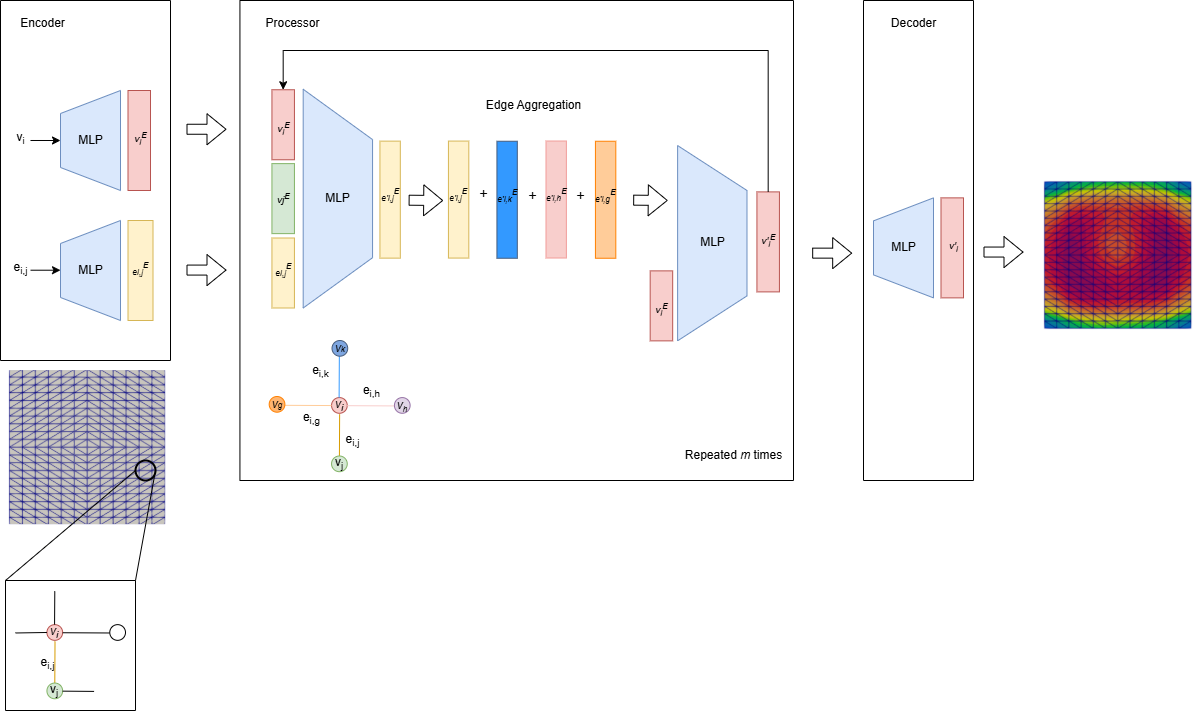
\includegraphics[width=\linewidth]{figures/surrogate_model.png}
	\caption{Mesh Graph Neural Network (MGNN) representing the surrogate model architecture.}
	\label{fig:surrogate_model}
\end{figure}

The MGNN architecture consists of three stages: encoder, processor, and decoder (Figure~\ref{fig:surrogate_model}). During the encoding stage, both node features $x_i$ and edge features $e_{ij}$ are mapped into their respective embedded representations, $v_i^E$ and $e_{ij}^E$. The processor stage performs message passing~\cite{battaglia2018relational} over the graph, where information is exchanged between nodes and their neighbors via the connecting edges over $m$ time steps, leading to iterative updates of the node embeddings $v_i^E$. Finally, in the decoding stage, the updated node embeddings are mapped to the model’s outputs, denoted by $v_i'$, which represent the network’s prediction at mesh vertex $i$.

The input vector of $\mathcal{S}$ consists of 254 features describing mesh node coordinates, sheet geometry (width, height, and thickness), material properties (volumetric heat capacity, emissivity, and thermal conductivity), pyrometer setpoints, lamp powers, and modulation parameters controlling the heating cycle.

The model outputs the predicted core temperature distribution over the mesh vertices together with four process-related quantities: energy consumption, heating time, and the maximum temperatures on the top and bottom surfaces of the sheet.

The encoder consists of two fully connected layers with 512 units, while the decoder consists of two fully connected layers with 128 units. ReLU activations are used throughout. The model is trained using the loss function $\mathcal{L}_s$ defined in Eq.~\ref{eq:loss_surrogate}, optimized with the Adam optimizer~\cite{kingma2014adam} using a learning rate of $1 \times 10^{-3}$ and a batch size of 64. Training is initially set to 1000 epochs, with early stopping applied based on the validation loss, resulting in convergence after 864 epochs.

The training was performed on a workstation equipped with an Intel Core i7 CPU, 16 GB of RAM, and an NVIDIA RTX A4000 GPU, requiring approximately four days.

\section{Loss function formulation}

The loss function adopted for the training of $\mathcal{S}$ balances temperature prediction accuracy and consistency of the process-related outputs. Let $\hat{\mathbf{y}} \in \mathbb{R}^{N \times d}$ denote the predicted outputs and $\mathbf{y}$ the corresponding ground truth, where $N$ is the number of mesh vertices and $d$ is the output dimension. The first component of the output corresponds to the temperature distribution $\hat{\mathbf{y}}_C$, while the remaining $d-1$ components correspond to the process-related outputs. The temperature distribution error is defined as the relative $\ell_2$ norm:

\begin{equation}
	E_T = \frac{\left\| \hat{\mathbf{y}}_C - \mathbf{y}_C \right\|_2}{\left\| \mathbf{y}_C \right\|_2}
\end{equation}

\noindent while the process-related outputs error is computed through the mean squared error:

\begin{equation}
	E_P = \sum_{k=2}^{d} \frac{1}{n} \sum_{i=1}^{n} \left( \hat{\mathbf{y}}_{i,k} - \mathbf{y}_{i,k} \right)^2
\end{equation}

A sigmoid weighting term is used to balance the contributions of $E_T$ and $E_P$ in the final loss:

\begin{equation}
	\sigma = \text{sigmoid} \left( \frac{E_T - \delta}{\tau \cdot \delta} \right)
\end{equation}

\noindent where $\delta = 0.003$ defines the acceptable relative $\ell_2$ error threshold and $\tau = 0.1$ controls the transition sharpness between the two loss regimes, both selected empirically based on preliminary experiments.

The final loss is defined as:

\begin{equation}
	\mathcal{L}_s = \sigma \cdot E_T + (1 - \sigma) \cdot \frac{1}{E_P + 1}
	\label{eq:loss_surrogate}
\end{equation}

This loss formulation adaptively prioritizes temperature distribution accuracy when errors are large, while maintaining consistency with process-related outputs once the temperature prediction is sufficiently accurate.

\section{Model assessment}

\begin{figure}[h]
	\centering
	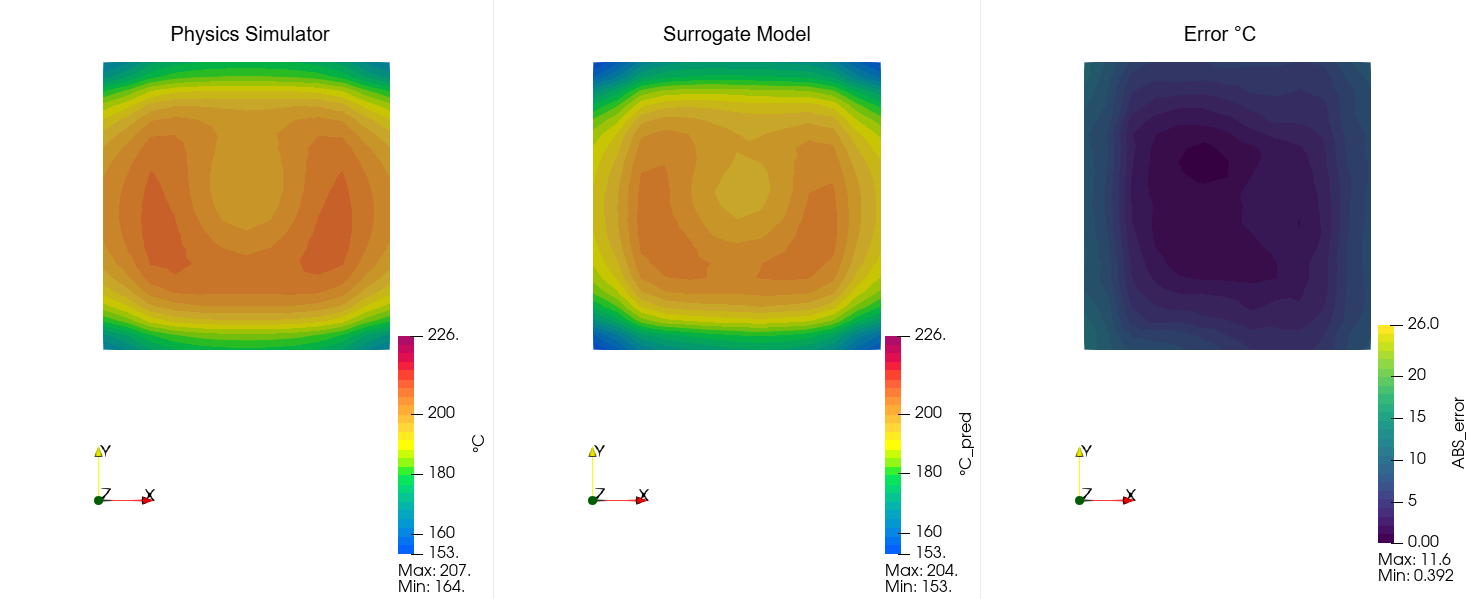
\includegraphics[width=0.7\linewidth]{figures/surrogate_model_with_label.png}
	\caption{Prediction example on the test set. From left to right: the temperature distribution obtained from the physics-based simulator, the prediction produced by the surrogate model and the absolute error between the target temperature distribution and the predicted one.}
	\label{fig:surrogate_model_prediction}
\end{figure}

At the end of training, evaluation of the temperature distribution reveals a maximum average absolute error of $1.23~^\circ\mathrm{C}$ on the training set, $3.43~^\circ\mathrm{C}$ on the validation set, and $9.65~^\circ\mathrm{C}$ on the test set.

Figure~\ref{fig:surrogate_model_prediction} shows an example prediction from the test set. In the example, the surrogate model preserves the spatial structure of the temperature field and correctly identifies regions of higher and lower temperature. The largest deviations occur along the left and right edges of the sheet, where the predicted temperature is slightly lower than the reference solution.

\begin{table}[b]
	\centering
	\footnotesize
	\caption{Physics-based simulator and surrogate model runtime for example.}
	\label{tab:surrogate_perf}
	\setlength{\tabcolsep}{5pt}
	\begin{tabular}{ccc}
		\toprule
		\textbf{Simulator (s)} & \textbf{Surrogate model (s)} & \textbf{Speed-up} \\
		\midrule
		$\approx 105.0$ & $\approx 0.70$ & \textbf{150$\times$} \\
		\bottomrule
	\end{tabular}
\end{table}

Table~\ref{tab:surrogate_perf} reports the processing times required by the physics-based simulator and the surrogate model for a single example. The surrogate model achieves a speed-up of 150$\times$ compared with the physics-based simulator. This reduction in computational time enables its integration into the machine control pipeline and improves the efficiency of training the inverse model, since the loss function is evaluated using temperature distributions generated from the predicted machine parameters.
